% a4 paper with title page on separate page
\documentclass[a4paper, titlepage]{article}
\usepackage{geometry}
\usepackage{graphicx}
\usepackage{todonotes}
% more date and time options
\usepackage{datetime}
% for only month and year in title
\newdateformat{monthyeardate}{\monthname[\THEMONTH] \THEYEAR}	

\title{Packet Processing in Java}
\author{Ashley Hemingway}
\date{\monthyeardate\today}

\begin{document}

\maketitle

%\todo{test1}
%\todo[noline]{test2}
%\todo[inline]{test3}
%\missingfigure{test4}

\listoftodos

\newpage

\tableofcontents

\newpage

\section{Introduction (1 - 3 pages)}
\subsection{Motivation}
As modern computing techniques advance, people are trying to find more generic solutions to problems which have been solved by native applications in the past. A main area of focus has been network middleboxes (network appliance), which are developed to manipulate network packets. Common examples of middleboxes are firewalls, network address translators (NATs) and load balancers, all of which inspect or transform network packets. In recent years, people have been developing a number of programmable middleboxes which allow these generic solutions to be used on a wide scale basis.

\begin{center}
	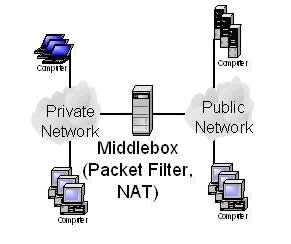
\includegraphics[scale=0.75]{images/middleboxes.jpg}
\end{center}

As middleboxes are mainly used for networking purposes, they are required to process network packets at line rate (i.e. at speeds which mean there is no backlog of packets to process). This requires the application to retrieve the packet from the network line, inspect and transform the packet in the desired way and then insert the packet back onto the network line, all within a time period sufficient enough to not cause a backlog. High performance implementations of such applications are available, but are written in native languages, predominately in C/C++. However, more and more high performance computing projects are been developed in Java and have succeeded in performing at similar speeds to C/C++ applications. \\
\newline
The main challenge is actually getting the I/O system for the Java application to run at line rate speeds, due to challenges with how the JVM (Java Virtual Machine) interacts with memory and the computer's kernel. Once this challenge has been overcome, there are no reasons why programmable middleboxes written in none native languages such as Java can exist within networking systems.

\subsection{Objectives}
\todo[inline]{More here about main objective I think - check slides - mention DPDK before and link to background}
With the main aim of implementing a Java application which can process network packets at line speed with similar comparisons to C/C++ applications we defined a number of milestone objectives:
\begin{itemize}
	\item Understand similar application and API's written in C/C++ which process at line speeds and how the implementations can be exploited for Java applications
	\item Exploit two Java features which allows for better I/O performance: ByteBuffer's and the Java Native Interface (JNI)
	\item Implement basic middlebox applications in Java such as a firewall and a NAT
	\item Compare Java implementations to those which are pure Java and pure C/C++
\end{itemize}

\subsection{Contributions / Main idea for solving it}

\newpage

\section{Background (10 - 20 pages)}
\subsection{Network Components}
\subsubsection{Network Packets}
A network packet is responsible for carrying data from a source to a destination. Packets are routed, fragmented and dropped via information stored within the packet's header. Note: in this report packets and datagrams are interchangeable.

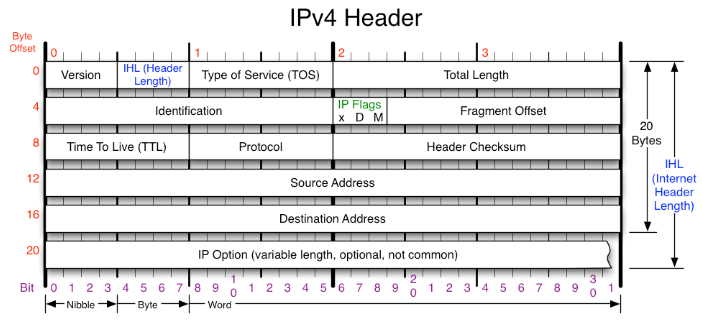
\includegraphics[width=\textwidth]{images/ipv4header.png}

\begin{itemize}
	\item Version - IP version number (set to 4 for IPv4)
	\item Internet Header Length (IHL) - Specifies the size of the header since a IPv4 header can be of varying length
	\item Type of Service (TOS) - As of RFC 2474 redefined to be differentiated services code point (DSCP) which is used by real time data streaming services like voice over IP (VoIP) and explicit congestion notification (ECN) which allows end-to-end notification of network congestion without dropping packets
	\item Total Length - Defines the entire packet size (header + data) in bytes. Min length is 20 bytes and max length is 65,535 bytes, although datagrams may be fragmented.
	\item Identification - Used for uniquely identifying the group of fragments of a single IP datagram
	\item X Flag - Reserved, must be zero
	\item DF Flag - If set, and fragmentation is required to route the packet, then the packet will be dropped. Usually occurs when packet destination doesn't have enough resources to handle incoming packet.
	\item MF Flag - If packet isn't fragmented, flag is clear. If packet is fragmented and datagram isn't the last fragment of the packet, the flag is set.
	\item Fragment Offset - Specifies the offset of a particular fragment relative to the beginning of the original unfragmented IP datagram
	\item Time To Live (TTL) - Limits the datagrams lifetime specified in seconds. In reality, this is actually the hop count which is decremented each time the datagram is routed. This helps to stop circular routing.
	\item Protocol - Defines the protocol used the data of the datagram
	\item Header Checksum - Used for to check for errors in the header. Router calculates checksum and compares to this value, discarding if they don't match.
	\item Source Address - Sender of the packet
	\item Destination Address - Receiver of the packet
	\item Options - specifies a number of options which are applicable for each datagram. As this project doesn't concern these it won't be discussed further.
\end{itemize}

\subsubsection{Network Address Translator (NAT)}
As a routing device, a NAT is responsible for remapping an IP address to another by altering the IP datagram packet header. NAT's have become extremely important in modern networking systems due to IPv4 address exhaustion, allowing a single public IP address to map to multiple private IP addresses. This is particularly useful in large corporations where only a limited public network connection is required, meaning that all private IP addresses (usually associated with a single machine) are mapped to the same public IP address. A NAT will make use of multiple connection ports to identify which packets are for which private IP address and then re-assign the packet header so the internal routers can forward the packet correctly. As can be seen by Figure (number) each internal address is mapped to via the port number associated with the external address. NAT's are generally implemented as part of a network firewall as they inspect the datagram packets for malicious data and sources.

\begin{center}
	\begin{tabular} { | c | c | }
		\hline
		\textbf{Private IP Address} & \textbf{Public IP Address} \\
		\hline
		10.0.0.1 & 14.1.23.5:62450 \\
		\hline
		10.0.0.2 & 14.1.23.5:62451 \\
		\hline
		10.0.0.3 & 14.1.23.5:62452 \\
		\hline
		10.0.0.4 & 14.1.23.5:62453 \\
		\hline
	\end{tabular}
\end{center}

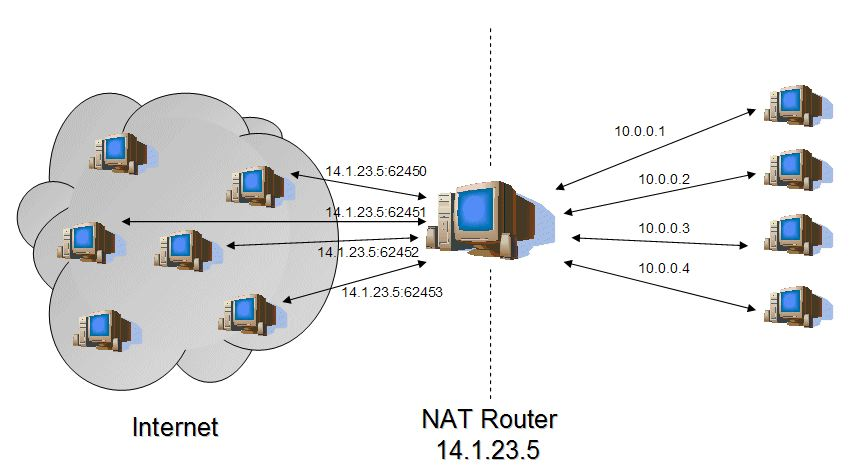
\includegraphics[width=\textwidth]{images/nat.jpg}

\subsubsection{Firewall}
Firewalls are generally the major applications which sits between the public and private network of a system. They provide packet filtering which controls which packets can enter the private network via establishing a set of rules which packets have to adhere to. Filtering can be based on a number attributes of the packet such as the source and destination IP address and port and the destination service. Firewalls can also offer a number of other useful features such as NAT's or dynamic host configuration protocol (DCHP). As well as providing protection on a network level, application layer firewalls exist which stop certain applications from sending or receiving a packet. \\
\newline
Within this project, the term 'firewall' is used for a network layer firewall which filters packets dependent on the source IP address. Any changes in this will be mentioned within the relevant sections.

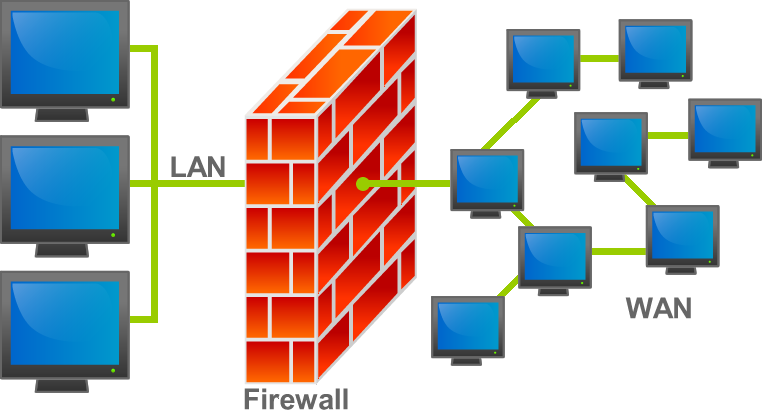
\includegraphics[width=\textwidth]{images/firewall.png}

\subsection{Java}
\subsubsection{JVM Networking}
\subsubsection{JNI}
\subsubsection{ByteBuffer}
\subsection{I/O API's}
\subsubsection{DPDK}
\subsubsection{Netmap}

\newpage

\section{Project Plan (1 - 2 pages)}
\subsection{Time Plan}
The given time plan outlined below provides me with a useful indication of how to measure the progress of the project, as well as dividing the whole project into smaller, more manageable sections which can be assessed individually. Some of the milestones have already been completed, while the others are expected to be finished within the given time period.
\subsubsection{Key Milestones}
\begin{itemize}
	\item Done - Background reading on DPDK \& Netmap
	\item Done - Understand workings off Java Native Interface (JNI) and Java memory
	\item Done - Get DPDK (and associated programs) working on local machine (or VM)
	\item In Progress - Link DPDK library with shared object files for JNI
	\item Awaiting - Implement basic IP address firewall
	\item Awaiting - Implement basic NAT
	\item Awaiting - Find similar implementations of firewall and NAT in C/C++ and Java
	\item Awaiting - Set up 2 independent machines to use for testing purposes
	\item Awaiting - Run tests on firewall and NAT to produces performance measurements
	\item Awaiting - Analyse results
\end{itemize}

\subsubsection{Time Estimations}
\missingfigure{Gantt chart would be very useful here}

\subsubsection{Completed Milestones}
As indicated, the background reading on the DPDK and Netmap libraries has been completed and the overview of the implementation has been assessed. The pros and cons has been outlined in the background section (give number). From this, I was able to get DPDL fully working on a virtual machine running locally on a personal machine, which allowed for a more in depth analysis of the implementation of DPDK. \\
\newline
I'm currently working on a way to generate shared object files from the C code used the link DPDK with a Java application. Due to the complex build system which DPDK makes use of, there has been a number of issues which have arisen.

\subsection{Fall Back Position}
If a number of unforeseen issues arise which impact on the progress of the project, I've outlined a few of the key milestones which can be omitted in order to allow the project to still be evaluated:
\begin{itemize}
	\item Implement basic NAT
	\item Find similar implementations of firewall and NAT in C/C++ and Java
	\item Run tests on firewall and NAT to produces performance measurements
\end{itemize}
Obviously, the emission of the above milestones will result in a less accurate evaluation of the overall project, but it's better than having nothing to evaluate in the end. As seen above, limiting the testing to one type of middlebox (only the firewall) can still give good results. This therefore reduces the need to look for an implementation for the NAT in Java and C/C++, while meaning less tests will have to be carried out. I feel that the remaining milestones are definitely key to the project in order for an adequate evaluation to be carried out.

\subsection{Possible Extensions}
If time allows, there are a number of possible extensions which can be undertaken to advance the project further forward and produce more data which can be evaluated later.

\subsubsection{Off Heap Java Memory}
In order for DPDK to handle packets correctly, it has to insert these packets onto the outgoing 'ring'. To do this, the Java application has to place its serialised objects into memory which DPDK can access. Under the current implementation, the Java application will directly place the packets onto the 'ring' using the direct ByteBuffer allocate feature. The other option is to use off heap java memory which DPDK can access and place onto the 'ring' automatically. This off heap memory is slightly slower than on heap memory but much faster than disk memory, while off heap memory stores object serialised and therefore ready for transmission in packets. \\
\newline
Altering the application to make use of off heap Java memory and then testing the results could potentially offer a new and faster way of high performance packet processing in Java.

\subsubsection{Limit Testing}
Another interesting extension could be to test the limitations of the NAT and firewall applications implemented within this project, and therefore limitations of the underlaying implementation. In terms of the project, the limitations could be on the max packet throughput which it can handle without having to buffer the incoming packets.

\newpage

\section{Evaluation Plan (1 - 2 pages)}
The sections below outline how the project will be evaluated in order to determine whether the initial objectives have been met and whether the final outcome can be deemed a success, even if it provides unexpected results.

\subsection{Experiments \& Outcomes}
The main measure of success will be from the experiments which are to be carried out. Using the high performance Java packet I/O application which is currently been developed as part of this project, it will be compared to similar, already existing applications written in pure Java and in C/C++. This comparison will consist of 2 parts, firstly an application for a NAT and secondly a simple IP address firewall. These similar applications will then be benchmarked against each other and the results analysed. \\
\newline
Benchmarking will consist of setting up 2 independent computers, most likely standalone machines, in order to take advantage of the ability to overwrite the Intel network card drivers as required by the DPDK API. Testing can the be carried out on the firewall and NAT implemented in the 3 different contexts, measuring the latency between the time sent and time received of the network packet. As the testing will be carried out on the same machines, linked to the same network there is unlikely to be much variation in the network latency. This means that the variation in the times will be from the system processing speeds. To account for minor variations in the computing performance of the system, numerous iterations of the same test will be carried out, then taking statistical averages will provide the best final results in order to analyse correctly. \\
\newline
Analysis of the results will be mainly carried out via the use of graphs which allow for easy comparison of results. The expected outcome is that the application developed from within this project is of similar speeds to applications coded directly in C/C++ and much faster than those coded in Java. This is mainly because the kernel will be bypassed, but the use of the Java Native Interface is expected to slow down certain aspects of the application. However, as long as speeds which coincide with those of the line rate are reached, this will be acceptable. There is the possibility that expected speeds are well above those that are actually measured. Although this isn't ideal, the project shouldn't be considered a failure as it will still provide very useful feedback as to where future investigations should be focussed on.

\subsection{Functionality}
The functionality of the application will be evaluated to make sure it provides those features that are required. This will be done by manually accessing whether the provided application is capable of doing the features that we outlined in the objectives. This can obviously be done by assessing the firewall and NAT applications.

\subsection{Usability}

\newpage

\todo[inline]{Add references}
\todo[inline]{Add figure labels}
\todo[inline]{Complete front page}
\todo[inline]{Do final read through}
\todo[inline]{Put through spell checker}
\todo[inline]{Other useful applications}
\todo[inline]{What font, size and line spacing?}

\begin{thebibliography}{99}
http://www.neclab.eu/Projects/midcom.htm \\
http://windowsitpro.com/networking/what-types-network-address-translation-nat-exist \\
%http://en.wikipedia.org/wiki/Firewall_(computing)#mediaviewer/File:Firewall.png
\end{thebibliography}

\end{document}  